%  !TeX  root  =  user_guide.tex 
%\subsection{Other core plugins}
\section{Autres extensions principales}

% when the revision of a section has been finalized, 
% comment out the following line:
% \updatedisclaimer

%The remaining core plugins are listed in Table \ref{tab:other_core}, along with references to 
%the chapters in this manual which cover their usage.
Les extensions principales restantes sont énumérées dans la Table \ref{tab:other_core},
accompagnées des références aux chapitres de ce manuel qui traitent de leur
utilisation.

\begin{table}[H]
\centering
 \begin{tabular}{|l|l|p{8cm}|}
\hline \textbf{Icône} & \textbf{Extension} & \textbf{Chapitre de référence}\\
\hline

\includegraphics[width=0.6cm]{diagram_overlay}
 & Diagramme de couche \index{extensions!diagramme} & Chapitre \ref{sec:diagram}\\
\hline

\includegraphics[width=0.6cm]{grass}
 & GRASS \index{extensions!\grass!boîte à outils} & Chapitre \ref{sec:grass} et Appendice \ref{appdx_grass_toolbox_modules}\\
 \hline
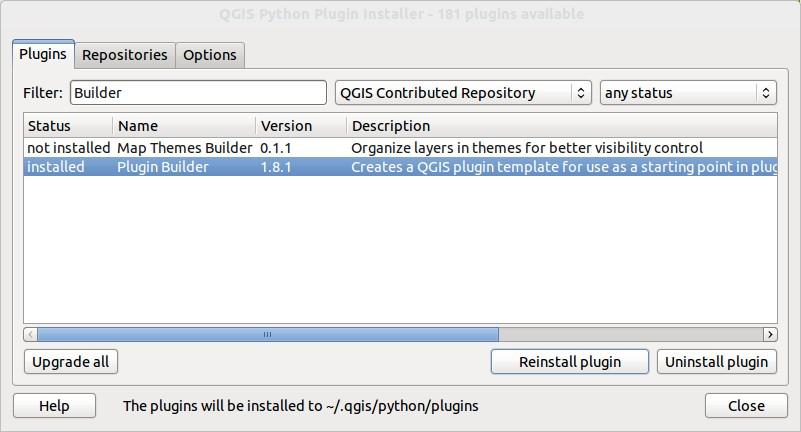
\includegraphics[width=0.6cm]{plugin_installer}
 & Installateur d'extensions \index{extensions!installation} & Chapitre \ref{sec:python_plugin_installer}\\
\hline

\includegraphics[width=0.6cm]{spiticon}
 & SPIT \index{extensions!spit} & Chapitre \ref{sec:loading_postgis_data} \\
 \hline

\includegraphics[width=0.6cm]{mIconAddWfsLayer}
 & WFS & Chapitre \ref{sec:ogc-wfs} \\
\hline
\end{tabular}
\caption{Autres extensions principales}\label{tab:other_core}
\end{table}
